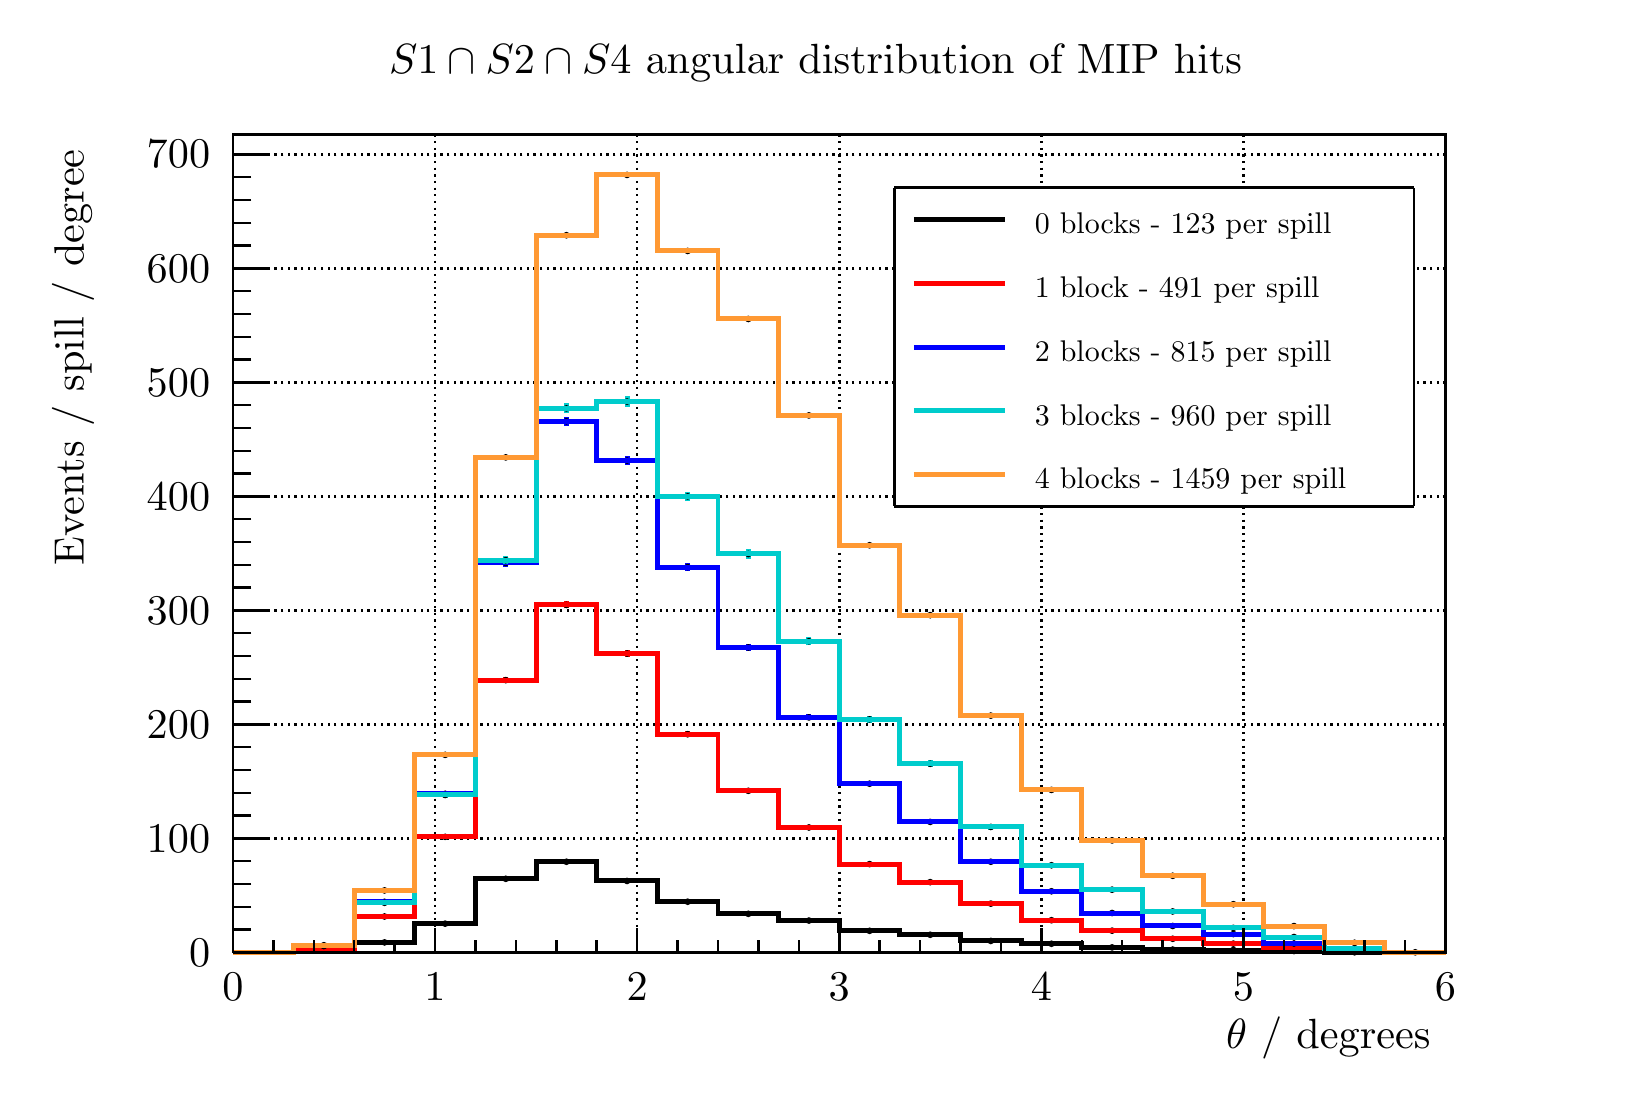
\begin{tikzpicture}
\pgfdeclareplotmark{cross} {
\pgfpathmoveto{\pgfpoint{-0.3\pgfplotmarksize}{\pgfplotmarksize}}
\pgfpathlineto{\pgfpoint{+0.3\pgfplotmarksize}{\pgfplotmarksize}}
\pgfpathlineto{\pgfpoint{+0.3\pgfplotmarksize}{0.3\pgfplotmarksize}}
\pgfpathlineto{\pgfpoint{+1\pgfplotmarksize}{0.3\pgfplotmarksize}}
\pgfpathlineto{\pgfpoint{+1\pgfplotmarksize}{-0.3\pgfplotmarksize}}
\pgfpathlineto{\pgfpoint{+0.3\pgfplotmarksize}{-0.3\pgfplotmarksize}}
\pgfpathlineto{\pgfpoint{+0.3\pgfplotmarksize}{-1.\pgfplotmarksize}}
\pgfpathlineto{\pgfpoint{-0.3\pgfplotmarksize}{-1.\pgfplotmarksize}}
\pgfpathlineto{\pgfpoint{-0.3\pgfplotmarksize}{-0.3\pgfplotmarksize}}
\pgfpathlineto{\pgfpoint{-1.\pgfplotmarksize}{-0.3\pgfplotmarksize}}
\pgfpathlineto{\pgfpoint{-1.\pgfplotmarksize}{0.3\pgfplotmarksize}}
\pgfpathlineto{\pgfpoint{-0.3\pgfplotmarksize}{0.3\pgfplotmarksize}}
\pgfpathclose
\pgfusepathqstroke
}
\pgfdeclareplotmark{cross*} {
\pgfpathmoveto{\pgfpoint{-0.3\pgfplotmarksize}{\pgfplotmarksize}}
\pgfpathlineto{\pgfpoint{+0.3\pgfplotmarksize}{\pgfplotmarksize}}
\pgfpathlineto{\pgfpoint{+0.3\pgfplotmarksize}{0.3\pgfplotmarksize}}
\pgfpathlineto{\pgfpoint{+1\pgfplotmarksize}{0.3\pgfplotmarksize}}
\pgfpathlineto{\pgfpoint{+1\pgfplotmarksize}{-0.3\pgfplotmarksize}}
\pgfpathlineto{\pgfpoint{+0.3\pgfplotmarksize}{-0.3\pgfplotmarksize}}
\pgfpathlineto{\pgfpoint{+0.3\pgfplotmarksize}{-1.\pgfplotmarksize}}
\pgfpathlineto{\pgfpoint{-0.3\pgfplotmarksize}{-1.\pgfplotmarksize}}
\pgfpathlineto{\pgfpoint{-0.3\pgfplotmarksize}{-0.3\pgfplotmarksize}}
\pgfpathlineto{\pgfpoint{-1.\pgfplotmarksize}{-0.3\pgfplotmarksize}}
\pgfpathlineto{\pgfpoint{-1.\pgfplotmarksize}{0.3\pgfplotmarksize}}
\pgfpathlineto{\pgfpoint{-0.3\pgfplotmarksize}{0.3\pgfplotmarksize}}
\pgfpathclose
\pgfusepathqfillstroke
}
\pgfdeclareplotmark{newstar} {
\pgfpathmoveto{\pgfqpoint{0pt}{\pgfplotmarksize}}
\pgfpathlineto{\pgfqpointpolar{44}{0.5\pgfplotmarksize}}
\pgfpathlineto{\pgfqpointpolar{18}{\pgfplotmarksize}}
\pgfpathlineto{\pgfqpointpolar{-20}{0.5\pgfplotmarksize}}
\pgfpathlineto{\pgfqpointpolar{-54}{\pgfplotmarksize}}
\pgfpathlineto{\pgfqpointpolar{-90}{0.5\pgfplotmarksize}}
\pgfpathlineto{\pgfqpointpolar{234}{\pgfplotmarksize}}
\pgfpathlineto{\pgfqpointpolar{198}{0.5\pgfplotmarksize}}
\pgfpathlineto{\pgfqpointpolar{162}{\pgfplotmarksize}}
\pgfpathlineto{\pgfqpointpolar{134}{0.5\pgfplotmarksize}}
\pgfpathclose
\pgfusepathqstroke
}
\pgfdeclareplotmark{newstar*} {
\pgfpathmoveto{\pgfqpoint{0pt}{\pgfplotmarksize}}
\pgfpathlineto{\pgfqpointpolar{44}{0.5\pgfplotmarksize}}
\pgfpathlineto{\pgfqpointpolar{18}{\pgfplotmarksize}}
\pgfpathlineto{\pgfqpointpolar{-20}{0.5\pgfplotmarksize}}
\pgfpathlineto{\pgfqpointpolar{-54}{\pgfplotmarksize}}
\pgfpathlineto{\pgfqpointpolar{-90}{0.5\pgfplotmarksize}}
\pgfpathlineto{\pgfqpointpolar{234}{\pgfplotmarksize}}
\pgfpathlineto{\pgfqpointpolar{198}{0.5\pgfplotmarksize}}
\pgfpathlineto{\pgfqpointpolar{162}{\pgfplotmarksize}}
\pgfpathlineto{\pgfqpointpolar{134}{0.5\pgfplotmarksize}}
\pgfpathclose
\pgfusepathqfillstroke
}
\definecolor{c}{rgb}{1,1,1};
\draw [color=c, fill=c] (0,0) rectangle (20,13.4957);
\draw [color=c, fill=c] (2.6,1.75444) rectangle (18,12.1461);
\definecolor{c}{rgb}{0,0,0};
\draw [c,line width=0.9] (2.6,1.75444) -- (2.6,12.1461) -- (18,12.1461) -- (18,1.75444) -- (2.6,1.75444);
\definecolor{c}{rgb}{1,1,1};
\draw [color=c, fill=c] (2.6,1.75444) rectangle (18,12.1461);
\definecolor{c}{rgb}{0,0,0};
\draw [c,line width=0.9] (2.6,1.75444) -- (2.6,12.1461) -- (18,12.1461) -- (18,1.75444) -- (2.6,1.75444);
\draw [c,line width=0.9] (2.6,1.75444) -- (18,1.75444);
\draw [c,dash pattern=on 0.80pt off 1.60pt ,line width=0.9] (2.6,12.1461) -- (2.6,1.75444);
\draw [c,dash pattern=on 0.80pt off 1.60pt ,line width=0.9] (5.16667,12.1461) -- (5.16667,1.75444);
\draw [c,dash pattern=on 0.80pt off 1.60pt ,line width=0.9] (7.73333,12.1461) -- (7.73333,1.75444);
\draw [c,dash pattern=on 0.80pt off 1.60pt ,line width=0.9] (10.3,12.1461) -- (10.3,1.75444);
\draw [c,dash pattern=on 0.80pt off 1.60pt ,line width=0.9] (12.8667,12.1461) -- (12.8667,1.75444);
\draw [c,dash pattern=on 0.80pt off 1.60pt ,line width=0.9] (15.4333,12.1461) -- (15.4333,1.75444);
\draw [c,dash pattern=on 0.80pt off 1.60pt ,line width=0.9] (18,12.1461) -- (18,1.75444);
\draw [c,line width=0.9] (2.6,1.75444) -- (2.6,12.1461);
\draw [c,dash pattern=on 0.80pt off 1.60pt ,line width=0.9] (18,1.75864) -- (2.6,1.75864);
\draw [c,dash pattern=on 0.80pt off 1.60pt ,line width=0.9] (18,3.20649) -- (2.6,3.20649);
\draw [c,dash pattern=on 0.80pt off 1.60pt ,line width=0.9] (18,4.65433) -- (2.6,4.65433);
\draw [c,dash pattern=on 0.80pt off 1.60pt ,line width=0.9] (18,6.10218) -- (2.6,6.10218);
\draw [c,dash pattern=on 0.80pt off 1.60pt ,line width=0.9] (18,7.55003) -- (2.6,7.55003);
\draw [c,dash pattern=on 0.80pt off 1.60pt ,line width=0.9] (18,8.99787) -- (2.6,8.99787);
\draw [c,dash pattern=on 0.80pt off 1.60pt ,line width=0.9] (18,10.4457) -- (2.6,10.4457);
\draw [c,dash pattern=on 0.80pt off 1.60pt ,line width=0.9] (18,11.8936) -- (2.6,11.8936);
\draw [c,dash pattern=on 0.80pt off 1.60pt ,line width=0.9] (18,1.75864) -- (2.6,1.75864);
\draw [c,dash pattern=on 0.80pt off 1.60pt ,line width=0.9] (18,11.8936) -- (2.6,11.8936);
\definecolor{c}{rgb}{0,0,0.6};
\draw [c,line width=0.9] (2.6,1.75864) -- (3.37,1.75864) -- (3.37,1.75864) -- (4.14,1.75864) -- (4.14,1.75864) -- (4.91,1.75864) -- (4.91,1.75864) -- (5.68,1.75864) -- (5.68,1.75864) -- (6.45,1.75864) -- (6.45,1.75864) -- (7.22,1.75864) --
 (7.22,1.75864) -- (7.99,1.75864) -- (7.99,1.75864) -- (8.76,1.75864) -- (8.76,1.75864) -- (9.53,1.75864) -- (9.53,1.75864) -- (10.3,1.75864) -- (10.3,1.75864) -- (11.07,1.75864) -- (11.07,1.75864) -- (11.84,1.75864) -- (11.84,1.75864) --
 (12.61,1.75864) -- (12.61,1.75864) -- (13.38,1.75864) -- (13.38,1.75864) -- (14.15,1.75864) -- (14.15,1.75864) -- (14.92,1.75864) -- (14.92,1.75864) -- (15.69,1.75864) -- (15.69,1.75864) -- (16.46,1.75864) -- (16.46,1.75864) -- (17.23,1.75864) --
 (17.23,1.75864) -- (18,1.75864);
\definecolor{c}{rgb}{0,0,0};
\draw [c,line width=0.9] (2.6,1.75444) -- (18,1.75444);
\draw [c,line width=0.9] (2.6,2.06619) -- (2.6,1.75444);
\draw [c,line width=0.9] (3.11333,1.91032) -- (3.11333,1.75444);
\draw [c,line width=0.9] (3.62667,1.91032) -- (3.62667,1.75444);
\draw [c,line width=0.9] (4.14,1.91032) -- (4.14,1.75444);
\draw [c,line width=0.9] (4.65333,1.91032) -- (4.65333,1.75444);
\draw [c,line width=0.9] (5.16667,2.06619) -- (5.16667,1.75444);
\draw [c,line width=0.9] (5.68,1.91032) -- (5.68,1.75444);
\draw [c,line width=0.9] (6.19333,1.91032) -- (6.19333,1.75444);
\draw [c,line width=0.9] (6.70667,1.91032) -- (6.70667,1.75444);
\draw [c,line width=0.9] (7.22,1.91032) -- (7.22,1.75444);
\draw [c,line width=0.9] (7.73333,2.06619) -- (7.73333,1.75444);
\draw [c,line width=0.9] (8.24667,1.91032) -- (8.24667,1.75444);
\draw [c,line width=0.9] (8.76,1.91032) -- (8.76,1.75444);
\draw [c,line width=0.9] (9.27333,1.91032) -- (9.27333,1.75444);
\draw [c,line width=0.9] (9.78667,1.91032) -- (9.78667,1.75444);
\draw [c,line width=0.9] (10.3,2.06619) -- (10.3,1.75444);
\draw [c,line width=0.9] (10.8133,1.91032) -- (10.8133,1.75444);
\draw [c,line width=0.9] (11.3267,1.91032) -- (11.3267,1.75444);
\draw [c,line width=0.9] (11.84,1.91032) -- (11.84,1.75444);
\draw [c,line width=0.9] (12.3533,1.91032) -- (12.3533,1.75444);
\draw [c,line width=0.9] (12.8667,2.06619) -- (12.8667,1.75444);
\draw [c,line width=0.9] (13.38,1.91032) -- (13.38,1.75444);
\draw [c,line width=0.9] (13.8933,1.91032) -- (13.8933,1.75444);
\draw [c,line width=0.9] (14.4067,1.91032) -- (14.4067,1.75444);
\draw [c,line width=0.9] (14.92,1.91032) -- (14.92,1.75444);
\draw [c,line width=0.9] (15.4333,2.06619) -- (15.4333,1.75444);
\draw [c,line width=0.9] (15.9467,1.91032) -- (15.9467,1.75444);
\draw [c,line width=0.9] (16.46,1.91032) -- (16.46,1.75444);
\draw [c,line width=0.9] (16.9733,1.91032) -- (16.9733,1.75444);
\draw [c,line width=0.9] (17.4867,1.91032) -- (17.4867,1.75444);
\draw [c,line width=0.9] (18,2.06619) -- (18,1.75444);
\draw [anchor=base] (2.6,1.14713) node[scale=1.52731, color=c, rotate=0]{0};
\draw [anchor=base] (5.16667,1.14713) node[scale=1.52731, color=c, rotate=0]{1};
\draw [anchor=base] (7.73333,1.14713) node[scale=1.52731, color=c, rotate=0]{2};
\draw [anchor=base] (10.3,1.14713) node[scale=1.52731, color=c, rotate=0]{3};
\draw [anchor=base] (12.8667,1.14713) node[scale=1.52731, color=c, rotate=0]{4};
\draw [anchor=base] (15.4333,1.14713) node[scale=1.52731, color=c, rotate=0]{5};
\draw [anchor=base] (18,1.14713) node[scale=1.52731, color=c, rotate=0]{6};
\draw [anchor= east] (18,0.674785) node[scale=1.52731, color=c, rotate=0]{$\theta$ / degrees};
\draw [c,line width=0.9] (2.6,1.75444) -- (2.6,12.1461);
\draw [c,line width=0.9] (3.062,1.75864) -- (2.6,1.75864);
\draw [c,line width=0.9] (2.831,2.04821) -- (2.6,2.04821);
\draw [c,line width=0.9] (2.831,2.33778) -- (2.6,2.33778);
\draw [c,line width=0.9] (2.831,2.62735) -- (2.6,2.62735);
\draw [c,line width=0.9] (2.831,2.91692) -- (2.6,2.91692);
\draw [c,line width=0.9] (3.062,3.20649) -- (2.6,3.20649);
\draw [c,line width=0.9] (2.831,3.49606) -- (2.6,3.49606);
\draw [c,line width=0.9] (2.831,3.78563) -- (2.6,3.78563);
\draw [c,line width=0.9] (2.831,4.0752) -- (2.6,4.0752);
\draw [c,line width=0.9] (2.831,4.36476) -- (2.6,4.36476);
\draw [c,line width=0.9] (3.062,4.65433) -- (2.6,4.65433);
\draw [c,line width=0.9] (2.831,4.9439) -- (2.6,4.9439);
\draw [c,line width=0.9] (2.831,5.23347) -- (2.6,5.23347);
\draw [c,line width=0.9] (2.831,5.52304) -- (2.6,5.52304);
\draw [c,line width=0.9] (2.831,5.81261) -- (2.6,5.81261);
\draw [c,line width=0.9] (3.062,6.10218) -- (2.6,6.10218);
\draw [c,line width=0.9] (2.831,6.39175) -- (2.6,6.39175);
\draw [c,line width=0.9] (2.831,6.68132) -- (2.6,6.68132);
\draw [c,line width=0.9] (2.831,6.97089) -- (2.6,6.97089);
\draw [c,line width=0.9] (2.831,7.26046) -- (2.6,7.26046);
\draw [c,line width=0.9] (3.062,7.55003) -- (2.6,7.55003);
\draw [c,line width=0.9] (2.831,7.8396) -- (2.6,7.8396);
\draw [c,line width=0.9] (2.831,8.12916) -- (2.6,8.12916);
\draw [c,line width=0.9] (2.831,8.41873) -- (2.6,8.41873);
\draw [c,line width=0.9] (2.831,8.7083) -- (2.6,8.7083);
\draw [c,line width=0.9] (3.062,8.99787) -- (2.6,8.99787);
\draw [c,line width=0.9] (2.831,9.28744) -- (2.6,9.28744);
\draw [c,line width=0.9] (2.831,9.57701) -- (2.6,9.57701);
\draw [c,line width=0.9] (2.831,9.86658) -- (2.6,9.86658);
\draw [c,line width=0.9] (2.831,10.1561) -- (2.6,10.1561);
\draw [c,line width=0.9] (3.062,10.4457) -- (2.6,10.4457);
\draw [c,line width=0.9] (2.831,10.7353) -- (2.6,10.7353);
\draw [c,line width=0.9] (2.831,11.0249) -- (2.6,11.0249);
\draw [c,line width=0.9] (2.831,11.3144) -- (2.6,11.3144);
\draw [c,line width=0.9] (2.831,11.604) -- (2.6,11.604);
\draw [c,line width=0.9] (3.062,11.8936) -- (2.6,11.8936);
\draw [c,line width=0.9] (3.062,1.75864) -- (2.6,1.75864);
\draw [c,line width=0.9] (3.062,11.8936) -- (2.6,11.8936);
\draw [anchor= east] (2.5,1.75864) node[scale=1.52731, color=c, rotate=0]{0};
\draw [anchor= east] (2.5,3.20649) node[scale=1.52731, color=c, rotate=0]{100};
\draw [anchor= east] (2.5,4.65433) node[scale=1.52731, color=c, rotate=0]{200};
\draw [anchor= east] (2.5,6.10218) node[scale=1.52731, color=c, rotate=0]{300};
\draw [anchor= east] (2.5,7.55003) node[scale=1.52731, color=c, rotate=0]{400};
\draw [anchor= east] (2.5,8.99787) node[scale=1.52731, color=c, rotate=0]{500};
\draw [anchor= east] (2.5,10.4457) node[scale=1.52731, color=c, rotate=0]{600};
\draw [anchor= east] (2.5,11.8936) node[scale=1.52731, color=c, rotate=0]{700};
\draw [anchor= east] (0.568481,12.1461) node[scale=1.52731, color=c, rotate=90]{Events / spill / degree};
\draw [c,line width=1.8] (3.755,1.78092) -- (3.755,1.78543);
\draw [c,line width=1.8] (3.755,1.78543) -- (3.755,1.78994);
\foreach \P in {(3.755,1.78543)}{\draw[mark options={color=c,fill=c},mark size=2.402402pt,mark=*,mark size=1pt] plot coordinates {\P};}
\draw [c,line width=1.8] (4.525,1.87622) -- (4.525,1.88556);
\draw [c,line width=1.8] (4.525,1.88556) -- (4.525,1.89489);
\foreach \P in {(4.525,1.88556)}{\draw[mark options={color=c,fill=c},mark size=2.402402pt,mark=*,mark size=1pt] plot coordinates {\P};}
\draw [c,line width=1.8] (5.295,2.1089) -- (5.295,2.12356);
\draw [c,line width=1.8] (5.295,2.12356) -- (5.295,2.13821);
\foreach \P in {(5.295,2.12356)}{\draw[mark options={color=c,fill=c},mark size=2.402402pt,mark=*,mark size=1pt] plot coordinates {\P};}
\draw [c,line width=1.8] (6.065,2.67124) -- (6.065,2.69332);
\draw [c,line width=1.8] (6.065,2.69332) -- (6.065,2.71539);
\foreach \P in {(6.065,2.69332)}{\draw[mark options={color=c,fill=c},mark size=2.402402pt,mark=*,mark size=1pt] plot coordinates {\P};}
\draw [c,line width=1.8] (6.835,2.88626) -- (6.835,2.91013);
\draw [c,line width=1.8] (6.835,2.91013) -- (6.835,2.93401);
\foreach \P in {(6.835,2.91013)}{\draw[mark options={color=c,fill=c},mark size=2.402402pt,mark=*,mark size=1pt] plot coordinates {\P};}
\draw [c,line width=1.8] (7.605,2.64479) -- (7.605,2.66625);
\draw [c,line width=1.8] (7.605,2.66625) -- (7.605,2.68771);
\foreach \P in {(7.605,2.66625)}{\draw[mark options={color=c,fill=c},mark size=2.402402pt,mark=*,mark size=1pt] plot coordinates {\P};}
\draw [c,line width=1.8] (8.375,2.38352) -- (8.375,2.40226);
\draw [c,line width=1.8] (8.375,2.40226) -- (8.375,2.42099);
\foreach \P in {(8.375,2.40226)}{\draw[mark options={color=c,fill=c},mark size=2.402402pt,mark=*,mark size=1pt] plot coordinates {\P};}
\draw [c,line width=1.8] (9.145,2.232) -- (9.145,2.2486);
\draw [c,line width=1.8] (9.145,2.2486) -- (9.145,2.26521);
\foreach \P in {(9.145,2.2486)}{\draw[mark options={color=c,fill=c},mark size=2.402402pt,mark=*,mark size=1pt] plot coordinates {\P};}
\draw [c,line width=1.8] (9.915,2.14767) -- (9.915,2.16297);
\draw [c,line width=1.8] (9.915,2.16297) -- (9.915,2.17827);
\foreach \P in {(9.915,2.16297)}{\draw[mark options={color=c,fill=c},mark size=2.402402pt,mark=*,mark size=1pt] plot coordinates {\P};}
\draw [c,line width=1.8] (10.685,2.01987) -- (10.685,2.03271);
\draw [c,line width=1.8] (10.685,2.03271) -- (10.685,2.04556);
\foreach \P in {(10.685,2.03271)}{\draw[mark options={color=c,fill=c},mark size=2.402402pt,mark=*,mark size=1pt] plot coordinates {\P};}
\draw [c,line width=1.8] (11.455,1.97084) -- (11.455,1.98245);
\draw [c,line width=1.8] (11.455,1.98245) -- (11.455,1.99405);
\foreach \P in {(11.455,1.98245)}{\draw[mark options={color=c,fill=c},mark size=2.402402pt,mark=*,mark size=1pt] plot coordinates {\P};}
\draw [c,line width=1.8] (12.225,1.89495) -- (12.225,1.90442);
\draw [c,line width=1.8] (12.225,1.90442) -- (12.225,1.9139);
\foreach \P in {(12.225,1.90442)}{\draw[mark options={color=c,fill=c},mark size=2.402402pt,mark=*,mark size=1pt] plot coordinates {\P};}
\draw [c,line width=1.8] (12.995,1.85993) -- (12.995,1.86849);
\draw [c,line width=1.8] (12.995,1.86849) -- (12.995,1.87705);
\foreach \P in {(12.995,1.86849)}{\draw[mark options={color=c,fill=c},mark size=2.402402pt,mark=*,mark size=1pt] plot coordinates {\P};}
\draw [c,line width=1.8] (13.765,1.81557) -- (13.765,1.82221);
\draw [c,line width=1.8] (13.765,1.82221) -- (13.765,1.82886);
\foreach \P in {(13.765,1.82221)}{\draw[mark options={color=c,fill=c},mark size=2.402402pt,mark=*,mark size=1pt] plot coordinates {\P};}
\draw [c,line width=1.8] (14.535,1.78947) -- (14.535,1.7947);
\draw [c,line width=1.8] (14.535,1.7947) -- (14.535,1.79993);
\foreach \P in {(14.535,1.7947)}{\draw[mark options={color=c,fill=c},mark size=2.402402pt,mark=*,mark size=1pt] plot coordinates {\P};}
\draw [c,line width=1.8] (15.305,1.78393) -- (15.305,1.78899);
\draw [c,line width=1.8] (15.305,1.78899) -- (15.305,1.79404);
\foreach \P in {(15.305,1.78899)}{\draw[mark options={color=c,fill=c},mark size=2.402402pt,mark=*,mark size=1pt] plot coordinates {\P};}
\draw [c,line width=1.8] (16.075,1.77233) -- (16.075,1.77629);
\draw [c,line width=1.8] (16.075,1.77629) -- (16.075,1.78025);
\foreach \P in {(16.075,1.77629)}{\draw[mark options={color=c,fill=c},mark size=2.402402pt,mark=*,mark size=1pt] plot coordinates {\P};}
\draw [c,line width=1.8] (16.845,1.75829) -- (16.845,1.76044);
\draw [c,line width=1.8] (16.845,1.76044) -- (16.845,1.7626);
\foreach \P in {(16.845,1.76044)}{\draw[mark options={color=c,fill=c},mark size=2.402402pt,mark=*,mark size=1pt] plot coordinates {\P};}
\draw [c,line width=1.8] (2.6,1.75864) -- (3.37,1.75864) -- (3.37,1.78543) -- (4.14,1.78543) -- (4.14,1.88556) -- (4.91,1.88556) -- (4.91,2.12356) -- (5.68,2.12356) -- (5.68,2.69332) -- (6.45,2.69332) -- (6.45,2.91013) -- (7.22,2.91013) --
 (7.22,2.66625) -- (7.99,2.66625) -- (7.99,2.40226) -- (8.76,2.40226) -- (8.76,2.2486) -- (9.53,2.2486) -- (9.53,2.16297) -- (10.3,2.16297) -- (10.3,2.03271) -- (11.07,2.03271) -- (11.07,1.98245) -- (11.84,1.98245) -- (11.84,1.90442) --
 (12.61,1.90442) -- (12.61,1.86849) -- (13.38,1.86849) -- (13.38,1.82221) -- (14.15,1.82221) -- (14.15,1.7947) -- (14.92,1.7947) -- (14.92,1.78899) -- (15.69,1.78899) -- (15.69,1.77629) -- (16.46,1.77629) -- (16.46,1.76044) -- (17.23,1.76044) --
 (17.23,1.75864) -- (18,1.75864);
\definecolor{c}{rgb}{1,0,0};
\draw [c,line width=1.8] (3.755,1.80493) -- (3.755,1.81036);
\draw [c,line width=1.8] (3.755,1.81036) -- (3.755,1.8158);
\definecolor{c}{rgb}{0,0,0};
\foreach \P in {(3.755,1.81036)}{\draw[mark options={color=c,fill=c},mark size=2.402402pt,mark=*,mark size=1pt] plot coordinates {\P};}
\definecolor{c}{rgb}{1,0,0};
\draw [c,line width=1.8] (4.525,2.19956) -- (4.525,2.21473);
\draw [c,line width=1.8] (4.525,2.21473) -- (4.525,2.2299);
\definecolor{c}{rgb}{0,0,0};
\foreach \P in {(4.525,2.21473)}{\draw[mark options={color=c,fill=c},mark size=2.402402pt,mark=*,mark size=1pt] plot coordinates {\P};}
\definecolor{c}{rgb}{1,0,0};
\draw [c,line width=1.8] (5.295,3.20012) -- (5.295,3.22614);
\draw [c,line width=1.8] (5.295,3.22614) -- (5.295,3.25215);
\definecolor{c}{rgb}{0,0,0};
\foreach \P in {(5.295,3.22614)}{\draw[mark options={color=c,fill=c},mark size=2.402402pt,mark=*,mark size=1pt] plot coordinates {\P};}
\definecolor{c}{rgb}{1,0,0};
\draw [c,line width=1.8] (6.065,5.17718) -- (6.065,5.21641);
\draw [c,line width=1.8] (6.065,5.21641) -- (6.065,5.25564);
\definecolor{c}{rgb}{0,0,0};
\foreach \P in {(6.065,5.21641)}{\draw[mark options={color=c,fill=c},mark size=2.402402pt,mark=*,mark size=1pt] plot coordinates {\P};}
\definecolor{c}{rgb}{1,0,0};
\draw [c,line width=1.8] (6.835,6.12751) -- (6.835,6.17155);
\draw [c,line width=1.8] (6.835,6.17155) -- (6.835,6.21559);
\definecolor{c}{rgb}{0,0,0};
\foreach \P in {(6.835,6.17155)}{\draw[mark options={color=c,fill=c},mark size=2.402402pt,mark=*,mark size=1pt] plot coordinates {\P};}
\definecolor{c}{rgb}{1,0,0};
\draw [c,line width=1.8] (7.605,5.51263) -- (7.605,5.55417);
\draw [c,line width=1.8] (7.605,5.55417) -- (7.605,5.59572);
\definecolor{c}{rgb}{0,0,0};
\foreach \P in {(7.605,5.55417)}{\draw[mark options={color=c,fill=c},mark size=2.402402pt,mark=*,mark size=1pt] plot coordinates {\P};}
\definecolor{c}{rgb}{1,0,0};
\draw [c,line width=1.8] (8.375,4.4935) -- (8.375,4.52942);
\draw [c,line width=1.8] (8.375,4.52942) -- (8.375,4.56533);
\definecolor{c}{rgb}{0,0,0};
\foreach \P in {(8.375,4.52942)}{\draw[mark options={color=c,fill=c},mark size=2.402402pt,mark=*,mark size=1pt] plot coordinates {\P};}
\definecolor{c}{rgb}{1,0,0};
\draw [c,line width=1.8] (9.145,3.77944) -- (9.145,3.81107);
\draw [c,line width=1.8] (9.145,3.81107) -- (9.145,3.8427);
\definecolor{c}{rgb}{0,0,0};
\foreach \P in {(9.145,3.81107)}{\draw[mark options={color=c,fill=c},mark size=2.402402pt,mark=*,mark size=1pt] plot coordinates {\P};}
\definecolor{c}{rgb}{1,0,0};
\draw [c,line width=1.8] (9.915,3.31728) -- (9.915,3.34528);
\draw [c,line width=1.8] (9.915,3.34528) -- (9.915,3.37327);
\definecolor{c}{rgb}{0,0,0};
\foreach \P in {(9.915,3.34528)}{\draw[mark options={color=c,fill=c},mark size=2.402402pt,mark=*,mark size=1pt] plot coordinates {\P};}
\definecolor{c}{rgb}{1,0,0};
\draw [c,line width=1.8] (10.685,2.85574) -- (10.685,2.87987);
\draw [c,line width=1.8] (10.685,2.87987) -- (10.685,2.90399);
\definecolor{c}{rgb}{0,0,0};
\foreach \P in {(10.685,2.87987)}{\draw[mark options={color=c,fill=c},mark size=2.402402pt,mark=*,mark size=1pt] plot coordinates {\P};}
\definecolor{c}{rgb}{1,0,0};
\draw [c,line width=1.8] (11.455,2.62933) -- (11.455,2.65105);
\draw [c,line width=1.8] (11.455,2.65105) -- (11.455,2.67276);
\definecolor{c}{rgb}{0,0,0};
\foreach \P in {(11.455,2.65105)}{\draw[mark options={color=c,fill=c},mark size=2.402402pt,mark=*,mark size=1pt] plot coordinates {\P};}
\definecolor{c}{rgb}{1,0,0};
\draw [c,line width=1.8] (12.225,2.35957) -- (12.225,2.37802);
\draw [c,line width=1.8] (12.225,2.37802) -- (12.225,2.39648);
\definecolor{c}{rgb}{0,0,0};
\foreach \P in {(12.225,2.37802)}{\draw[mark options={color=c,fill=c},mark size=2.402402pt,mark=*,mark size=1pt] plot coordinates {\P};}
\definecolor{c}{rgb}{1,0,0};
\draw [c,line width=1.8] (12.995,2.15181) -- (12.995,2.16737);
\draw [c,line width=1.8] (12.995,2.16737) -- (12.995,2.18293);
\definecolor{c}{rgb}{0,0,0};
\foreach \P in {(12.995,2.16737)}{\draw[mark options={color=c,fill=c},mark size=2.402402pt,mark=*,mark size=1pt] plot coordinates {\P};}
\definecolor{c}{rgb}{1,0,0};
\draw [c,line width=1.8] (13.765,2.02139) -- (13.765,2.03475);
\draw [c,line width=1.8] (13.765,2.03475) -- (13.765,2.04812);
\definecolor{c}{rgb}{0,0,0};
\foreach \P in {(13.765,2.03475)}{\draw[mark options={color=c,fill=c},mark size=2.402402pt,mark=*,mark size=1pt] plot coordinates {\P};}
\definecolor{c}{rgb}{1,0,0};
\draw [c,line width=1.8] (14.535,1.92091) -- (14.535,1.93159);
\draw [c,line width=1.8] (14.535,1.93159) -- (14.535,1.94228);
\definecolor{c}{rgb}{0,0,0};
\foreach \P in {(14.535,1.93159)}{\draw[mark options={color=c,fill=c},mark size=2.402402pt,mark=*,mark size=1pt] plot coordinates {\P};}
\definecolor{c}{rgb}{1,0,0};
\draw [c,line width=1.8] (15.305,1.86103) -- (15.305,1.8702);
\draw [c,line width=1.8] (15.305,1.8702) -- (15.305,1.87938);
\definecolor{c}{rgb}{0,0,0};
\foreach \P in {(15.305,1.8702)}{\draw[mark options={color=c,fill=c},mark size=2.402402pt,mark=*,mark size=1pt] plot coordinates {\P};}
\definecolor{c}{rgb}{1,0,0};
\draw [c,line width=1.8] (16.075,1.81353) -- (16.075,1.82129);
\draw [c,line width=1.8] (16.075,1.82129) -- (16.075,1.82905);
\definecolor{c}{rgb}{0,0,0};
\foreach \P in {(16.075,1.82129)}{\draw[mark options={color=c,fill=c},mark size=2.402402pt,mark=*,mark size=1pt] plot coordinates {\P};}
\definecolor{c}{rgb}{1,0,0};
\draw [c,line width=1.8] (16.845,1.7621) -- (16.845,1.76623);
\draw [c,line width=1.8] (16.845,1.76623) -- (16.845,1.77036);
\definecolor{c}{rgb}{0,0,0};
\foreach \P in {(16.845,1.76623)}{\draw[mark options={color=c,fill=c},mark size=2.402402pt,mark=*,mark size=1pt] plot coordinates {\P};}
\definecolor{c}{rgb}{1,0,0};
\draw [c,line width=1.8] (2.6,1.75864) -- (3.37,1.75864) -- (3.37,1.81036) -- (4.14,1.81036) -- (4.14,2.21473) -- (4.91,2.21473) -- (4.91,3.22614) -- (5.68,3.22614) -- (5.68,5.21641) -- (6.45,5.21641) -- (6.45,6.17155) -- (7.22,6.17155) --
 (7.22,5.55417) -- (7.99,5.55417) -- (7.99,4.52942) -- (8.76,4.52942) -- (8.76,3.81107) -- (9.53,3.81107) -- (9.53,3.34528) -- (10.3,3.34528) -- (10.3,2.87987) -- (11.07,2.87987) -- (11.07,2.65105) -- (11.84,2.65105) -- (11.84,2.37802) --
 (12.61,2.37802) -- (12.61,2.16737) -- (13.38,2.16737) -- (13.38,2.03475) -- (14.15,2.03475) -- (14.15,1.93159) -- (14.92,1.93159) -- (14.92,1.8702) -- (15.69,1.8702) -- (15.69,1.82129) -- (16.46,1.82129) -- (16.46,1.76623) -- (17.23,1.76623) --
 (17.23,1.75864) -- (18,1.75864);
\definecolor{c}{rgb}{0,0,1};
\draw [c,line width=1.8] (3.755,1.8349) -- (3.755,1.84212);
\draw [c,line width=1.8] (3.755,1.84212) -- (3.755,1.84934);
\definecolor{c}{rgb}{0,0,0};
\foreach \P in {(3.755,1.84212)}{\draw[mark options={color=c,fill=c},mark size=2.402402pt,mark=*,mark size=1pt] plot coordinates {\P};}
\definecolor{c}{rgb}{0,0,1};
\draw [c,line width=1.8] (4.525,2.38243) -- (4.525,2.40101);
\draw [c,line width=1.8] (4.525,2.40101) -- (4.525,2.41959);
\definecolor{c}{rgb}{0,0,0};
\foreach \P in {(4.525,2.40101)}{\draw[mark options={color=c,fill=c},mark size=2.402402pt,mark=*,mark size=1pt] plot coordinates {\P};}
\definecolor{c}{rgb}{0,0,1};
\draw [c,line width=1.8] (5.295,3.74137) -- (5.295,3.77281);
\draw [c,line width=1.8] (5.295,3.77281) -- (5.295,3.80426);
\definecolor{c}{rgb}{0,0,0};
\foreach \P in {(5.295,3.77281)}{\draw[mark options={color=c,fill=c},mark size=2.402402pt,mark=*,mark size=1pt] plot coordinates {\P};}
\definecolor{c}{rgb}{0,0,1};
\draw [c,line width=1.8] (6.065,6.65657) -- (6.065,6.7044);
\draw [c,line width=1.8] (6.065,6.7044) -- (6.065,6.75223);
\definecolor{c}{rgb}{0,0,0};
\foreach \P in {(6.065,6.7044)}{\draw[mark options={color=c,fill=c},mark size=2.402402pt,mark=*,mark size=1pt] plot coordinates {\P};}
\definecolor{c}{rgb}{0,0,1};
\draw [c,line width=1.8] (6.835,8.44848) -- (6.835,8.50348);
\draw [c,line width=1.8] (6.835,8.50348) -- (6.835,8.55847);
\definecolor{c}{rgb}{0,0,0};
\foreach \P in {(6.835,8.50348)}{\draw[mark options={color=c,fill=c},mark size=2.402402pt,mark=*,mark size=1pt] plot coordinates {\P};}
\definecolor{c}{rgb}{0,0,1};
\draw [c,line width=1.8] (7.605,7.95202) -- (7.605,8.00527);
\draw [c,line width=1.8] (7.605,8.00527) -- (7.605,8.05852);
\definecolor{c}{rgb}{0,0,0};
\foreach \P in {(7.605,8.00527)}{\draw[mark options={color=c,fill=c},mark size=2.402402pt,mark=*,mark size=1pt] plot coordinates {\P};}
\definecolor{c}{rgb}{0,0,1};
\draw [c,line width=1.8] (8.375,6.60381) -- (8.375,6.65181);
\draw [c,line width=1.8] (8.375,6.65181) -- (8.375,6.69981);
\definecolor{c}{rgb}{0,0,0};
\foreach \P in {(8.375,6.65181)}{\draw[mark options={color=c,fill=c},mark size=2.402402pt,mark=*,mark size=1pt] plot coordinates {\P};}
\definecolor{c}{rgb}{0,0,1};
\draw [c,line width=1.8] (9.145,5.58771) -- (9.145,5.63139);
\draw [c,line width=1.8] (9.145,5.63139) -- (9.145,5.67506);
\definecolor{c}{rgb}{0,0,0};
\foreach \P in {(9.145,5.63139)}{\draw[mark options={color=c,fill=c},mark size=2.402402pt,mark=*,mark size=1pt] plot coordinates {\P};}
\definecolor{c}{rgb}{0,0,1};
\draw [c,line width=1.8] (9.915,4.70424) -- (9.915,4.74288);
\draw [c,line width=1.8] (9.915,4.74288) -- (9.915,4.78153);
\definecolor{c}{rgb}{0,0,0};
\foreach \P in {(9.915,4.74288)}{\draw[mark options={color=c,fill=c},mark size=2.402402pt,mark=*,mark size=1pt] plot coordinates {\P};}
\definecolor{c}{rgb}{0,0,1};
\draw [c,line width=1.8] (10.685,3.86779) -- (10.685,3.90134);
\draw [c,line width=1.8] (10.685,3.90134) -- (10.685,3.93489);
\definecolor{c}{rgb}{0,0,0};
\foreach \P in {(10.685,3.90134)}{\draw[mark options={color=c,fill=c},mark size=2.402402pt,mark=*,mark size=1pt] plot coordinates {\P};}
\definecolor{c}{rgb}{0,0,1};
\draw [c,line width=1.8] (11.455,3.38639) -- (11.455,3.41609);
\draw [c,line width=1.8] (11.455,3.41609) -- (11.455,3.44579);
\definecolor{c}{rgb}{0,0,0};
\foreach \P in {(11.455,3.41609)}{\draw[mark options={color=c,fill=c},mark size=2.402402pt,mark=*,mark size=1pt] plot coordinates {\P};}
\definecolor{c}{rgb}{0,0,1};
\draw [c,line width=1.8] (12.225,2.88474) -- (12.225,2.90996);
\draw [c,line width=1.8] (12.225,2.90996) -- (12.225,2.93519);
\definecolor{c}{rgb}{0,0,0};
\foreach \P in {(12.225,2.90996)}{\draw[mark options={color=c,fill=c},mark size=2.402402pt,mark=*,mark size=1pt] plot coordinates {\P};}
\definecolor{c}{rgb}{0,0,1};
\draw [c,line width=1.8] (12.995,2.51324) -- (12.995,2.53489);
\draw [c,line width=1.8] (12.995,2.53489) -- (12.995,2.55653);
\definecolor{c}{rgb}{0,0,0};
\foreach \P in {(12.995,2.53489)}{\draw[mark options={color=c,fill=c},mark size=2.402402pt,mark=*,mark size=1pt] plot coordinates {\P};}
\definecolor{c}{rgb}{0,0,1};
\draw [c,line width=1.8] (13.765,2.24093) -- (13.765,2.25892);
\draw [c,line width=1.8] (13.765,2.25892) -- (13.765,2.27691);
\definecolor{c}{rgb}{0,0,0};
\foreach \P in {(13.765,2.25892)}{\draw[mark options={color=c,fill=c},mark size=2.402402pt,mark=*,mark size=1pt] plot coordinates {\P};}
\definecolor{c}{rgb}{0,0,1};
\draw [c,line width=1.8] (14.535,2.07906) -- (14.535,2.09445);
\draw [c,line width=1.8] (14.535,2.09445) -- (14.535,2.10984);
\definecolor{c}{rgb}{0,0,0};
\foreach \P in {(14.535,2.09445)}{\draw[mark options={color=c,fill=c},mark size=2.402402pt,mark=*,mark size=1pt] plot coordinates {\P};}
\definecolor{c}{rgb}{0,0,1};
\draw [c,line width=1.8] (15.305,1.97778) -- (15.305,1.99132);
\draw [c,line width=1.8] (15.305,1.99132) -- (15.305,2.00485);
\definecolor{c}{rgb}{0,0,0};
\foreach \P in {(15.305,1.99132)}{\draw[mark options={color=c,fill=c},mark size=2.402402pt,mark=*,mark size=1pt] plot coordinates {\P};}
\definecolor{c}{rgb}{0,0,1};
\draw [c,line width=1.8] (16.075,1.86128) -- (16.075,1.87172);
\draw [c,line width=1.8] (16.075,1.87172) -- (16.075,1.88215);
\definecolor{c}{rgb}{0,0,0};
\foreach \P in {(16.075,1.87172)}{\draw[mark options={color=c,fill=c},mark size=2.402402pt,mark=*,mark size=1pt] plot coordinates {\P};}
\definecolor{c}{rgb}{0,0,1};
\draw [c,line width=1.8] (16.845,1.78537) -- (16.845,1.79238);
\draw [c,line width=1.8] (16.845,1.79238) -- (16.845,1.79939);
\definecolor{c}{rgb}{0,0,0};
\foreach \P in {(16.845,1.79238)}{\draw[mark options={color=c,fill=c},mark size=2.402402pt,mark=*,mark size=1pt] plot coordinates {\P};}
\definecolor{c}{rgb}{0,0,1};
\draw [c,line width=1.8] (2.6,1.75864) -- (3.37,1.75864) -- (3.37,1.84212) -- (4.14,1.84212) -- (4.14,2.40101) -- (4.91,2.40101) -- (4.91,3.77281) -- (5.68,3.77281) -- (5.68,6.7044) -- (6.45,6.7044) -- (6.45,8.50348) -- (7.22,8.50348) --
 (7.22,8.00527) -- (7.99,8.00527) -- (7.99,6.65181) -- (8.76,6.65181) -- (8.76,5.63139) -- (9.53,5.63139) -- (9.53,4.74288) -- (10.3,4.74288) -- (10.3,3.90134) -- (11.07,3.90134) -- (11.07,3.41609) -- (11.84,3.41609) -- (11.84,2.90996) --
 (12.61,2.90996) -- (12.61,2.53489) -- (13.38,2.53489) -- (13.38,2.25892) -- (14.15,2.25892) -- (14.15,2.09445) -- (14.92,2.09445) -- (14.92,1.99132) -- (15.69,1.99132) -- (15.69,1.87172) -- (16.46,1.87172) -- (16.46,1.79238) -- (17.23,1.79238) --
 (17.23,1.75864) -- (18,1.75864);
\definecolor{c}{rgb}{0,0.8,0.8};
\draw [c,line width=1.8] (3.755,1.83218) -- (3.755,1.84038);
\draw [c,line width=1.8] (3.755,1.84038) -- (3.755,1.84859);
\definecolor{c}{rgb}{0,0,0};
\foreach \P in {(3.755,1.84038)}{\draw[mark options={color=c,fill=c},mark size=2.402402pt,mark=*,mark size=1pt] plot coordinates {\P};}
\definecolor{c}{rgb}{0,0.8,0.8};
\draw [c,line width=1.8] (4.525,2.36748) -- (4.525,2.38868);
\draw [c,line width=1.8] (4.525,2.38868) -- (4.525,2.40987);
\definecolor{c}{rgb}{0,0,0};
\foreach \P in {(4.525,2.38868)}{\draw[mark options={color=c,fill=c},mark size=2.402402pt,mark=*,mark size=1pt] plot coordinates {\P};}
\definecolor{c}{rgb}{0,0.8,0.8};
\draw [c,line width=1.8] (5.295,3.72187) -- (5.295,3.75777);
\draw [c,line width=1.8] (5.295,3.75777) -- (5.295,3.79367);
\definecolor{c}{rgb}{0,0,0};
\foreach \P in {(5.295,3.75777)}{\draw[mark options={color=c,fill=c},mark size=2.402402pt,mark=*,mark size=1pt] plot coordinates {\P};}
\definecolor{c}{rgb}{0,0.8,0.8};
\draw [c,line width=1.8] (6.065,6.68513) -- (6.065,6.74018);
\draw [c,line width=1.8] (6.065,6.74018) -- (6.065,6.79522);
\definecolor{c}{rgb}{0,0,0};
\foreach \P in {(6.065,6.74018)}{\draw[mark options={color=c,fill=c},mark size=2.402402pt,mark=*,mark size=1pt] plot coordinates {\P};}
\definecolor{c}{rgb}{0,0.8,0.8};
\draw [c,line width=1.8] (6.835,8.60384) -- (6.835,8.66764);
\draw [c,line width=1.8] (6.835,8.66764) -- (6.835,8.73145);
\definecolor{c}{rgb}{0,0,0};
\foreach \P in {(6.835,8.66764)}{\draw[mark options={color=c,fill=c},mark size=2.402402pt,mark=*,mark size=1pt] plot coordinates {\P};}
\definecolor{c}{rgb}{0,0.8,0.8};
\draw [c,line width=1.8] (7.605,8.68881) -- (7.605,8.75426);
\draw [c,line width=1.8] (7.605,8.75426) -- (7.605,8.81971);
\definecolor{c}{rgb}{0,0,0};
\foreach \P in {(7.605,8.75426)}{\draw[mark options={color=c,fill=c},mark size=2.402402pt,mark=*,mark size=1pt] plot coordinates {\P};}
\definecolor{c}{rgb}{0,0.8,0.8};
\draw [c,line width=1.8] (8.375,7.48956) -- (8.375,7.55059);
\draw [c,line width=1.8] (8.375,7.55059) -- (8.375,7.61162);
\definecolor{c}{rgb}{0,0,0};
\foreach \P in {(8.375,7.55059)}{\draw[mark options={color=c,fill=c},mark size=2.402402pt,mark=*,mark size=1pt] plot coordinates {\P};}
\definecolor{c}{rgb}{0,0.8,0.8};
\draw [c,line width=1.8] (9.145,6.7598) -- (9.145,6.8186);
\draw [c,line width=1.8] (9.145,6.8186) -- (9.145,6.87739);
\definecolor{c}{rgb}{0,0,0};
\foreach \P in {(9.145,6.8186)}{\draw[mark options={color=c,fill=c},mark size=2.402402pt,mark=*,mark size=1pt] plot coordinates {\P};}
\definecolor{c}{rgb}{0,0.8,0.8};
\draw [c,line width=1.8] (9.915,5.65787) -- (9.915,5.7107);
\draw [c,line width=1.8] (9.915,5.7107) -- (9.915,5.76353);
\definecolor{c}{rgb}{0,0,0};
\foreach \P in {(9.915,5.7107)}{\draw[mark options={color=c,fill=c},mark size=2.402402pt,mark=*,mark size=1pt] plot coordinates {\P};}
\definecolor{c}{rgb}{0,0.8,0.8};
\draw [c,line width=1.8] (10.685,4.6716) -- (10.685,4.71844);
\draw [c,line width=1.8] (10.685,4.71844) -- (10.685,4.76527);
\definecolor{c}{rgb}{0,0,0};
\foreach \P in {(10.685,4.71844)}{\draw[mark options={color=c,fill=c},mark size=2.402402pt,mark=*,mark size=1pt] plot coordinates {\P};}
\definecolor{c}{rgb}{0,0.8,0.8};
\draw [c,line width=1.8] (11.455,4.11107) -- (11.455,4.1544);
\draw [c,line width=1.8] (11.455,4.1544) -- (11.455,4.19774);
\definecolor{c}{rgb}{0,0,0};
\foreach \P in {(11.455,4.1544)}{\draw[mark options={color=c,fill=c},mark size=2.402402pt,mark=*,mark size=1pt] plot coordinates {\P};}
\definecolor{c}{rgb}{0,0.8,0.8};
\draw [c,line width=1.8] (12.225,3.31667) -- (12.225,3.35221);
\draw [c,line width=1.8] (12.225,3.35221) -- (12.225,3.38776);
\definecolor{c}{rgb}{0,0,0};
\foreach \P in {(12.225,3.35221)}{\draw[mark options={color=c,fill=c},mark size=2.402402pt,mark=*,mark size=1pt] plot coordinates {\P};}
\definecolor{c}{rgb}{0,0.8,0.8};
\draw [c,line width=1.8] (12.995,2.83454) -- (12.995,2.86535);
\draw [c,line width=1.8] (12.995,2.86535) -- (12.995,2.89616);
\definecolor{c}{rgb}{0,0,0};
\foreach \P in {(12.995,2.86535)}{\draw[mark options={color=c,fill=c},mark size=2.402402pt,mark=*,mark size=1pt] plot coordinates {\P};}
\definecolor{c}{rgb}{0,0.8,0.8};
\draw [c,line width=1.8] (13.765,2.52705) -- (13.765,2.55504);
\draw [c,line width=1.8] (13.765,2.55504) -- (13.765,2.58304);
\definecolor{c}{rgb}{0,0,0};
\foreach \P in {(13.765,2.55504)}{\draw[mark options={color=c,fill=c},mark size=2.402402pt,mark=*,mark size=1pt] plot coordinates {\P};}
\definecolor{c}{rgb}{0,0.8,0.8};
\draw [c,line width=1.8] (14.535,2.2553) -- (14.535,2.27875);
\draw [c,line width=1.8] (14.535,2.27875) -- (14.535,2.30219);
\definecolor{c}{rgb}{0,0,0};
\foreach \P in {(14.535,2.27875)}{\draw[mark options={color=c,fill=c},mark size=2.402402pt,mark=*,mark size=1pt] plot coordinates {\P};}
\definecolor{c}{rgb}{0,0.8,0.8};
\draw [c,line width=1.8] (15.305,2.05046) -- (15.305,2.07004);
\draw [c,line width=1.8] (15.305,2.07004) -- (15.305,2.08963);
\definecolor{c}{rgb}{0,0,0};
\foreach \P in {(15.305,2.07004)}{\draw[mark options={color=c,fill=c},mark size=2.402402pt,mark=*,mark size=1pt] plot coordinates {\P};}
\definecolor{c}{rgb}{0,0.8,0.8};
\draw [c,line width=1.8] (16.075,1.93653) -- (16.075,1.95401);
\draw [c,line width=1.8] (16.075,1.95401) -- (16.075,1.9715);
\definecolor{c}{rgb}{0,0,0};
\foreach \P in {(16.075,1.95401)}{\draw[mark options={color=c,fill=c},mark size=2.402402pt,mark=*,mark size=1pt] plot coordinates {\P};}
\definecolor{c}{rgb}{0,0.8,0.8};
\draw [c,line width=1.8] (16.845,1.7994) -- (16.845,1.80979);
\draw [c,line width=1.8] (16.845,1.80979) -- (16.845,1.82018);
\definecolor{c}{rgb}{0,0,0};
\foreach \P in {(16.845,1.80979)}{\draw[mark options={color=c,fill=c},mark size=2.402402pt,mark=*,mark size=1pt] plot coordinates {\P};}
\definecolor{c}{rgb}{0,0.8,0.8};
\draw [c,line width=1.8] (17.615,1.75444) -- (17.615,1.76002);
\draw [c,line width=1.8] (17.615,1.76002) -- (17.615,1.7656);
\definecolor{c}{rgb}{0,0,0};
\foreach \P in {(17.615,1.76002)}{\draw[mark options={color=c,fill=c},mark size=2.402402pt,mark=*,mark size=1pt] plot coordinates {\P};}
\definecolor{c}{rgb}{0,0.8,0.8};
\draw [c,line width=1.8] (2.6,1.75864) -- (3.37,1.75864) -- (3.37,1.84038) -- (4.14,1.84038) -- (4.14,2.38868) -- (4.91,2.38868) -- (4.91,3.75777) -- (5.68,3.75777) -- (5.68,6.74018) -- (6.45,6.74018) -- (6.45,8.66764) -- (7.22,8.66764) --
 (7.22,8.75426) -- (7.99,8.75426) -- (7.99,7.55059) -- (8.76,7.55059) -- (8.76,6.8186) -- (9.53,6.8186) -- (9.53,5.7107) -- (10.3,5.7107) -- (10.3,4.71844) -- (11.07,4.71844) -- (11.07,4.1544) -- (11.84,4.1544) -- (11.84,3.35221) -- (12.61,3.35221)
 -- (12.61,2.86535) -- (13.38,2.86535) -- (13.38,2.55504) -- (14.15,2.55504) -- (14.15,2.27875) -- (14.92,2.27875) -- (14.92,2.07004) -- (15.69,2.07004) -- (15.69,1.95401) -- (16.46,1.95401) -- (16.46,1.80979) -- (17.23,1.80979) -- (17.23,1.76002) --
 (18,1.76002);
\definecolor{c}{rgb}{1,0.6,0.2};
\draw [c,line width=1.8] (3.755,1.84726) -- (3.755,1.84968);
\draw [c,line width=1.8] (3.755,1.84968) -- (3.755,1.8521);
\definecolor{c}{rgb}{0,0,0};
\foreach \P in {(3.755,1.84968)}{\draw[mark options={color=c,fill=c},mark size=2.402402pt,mark=*,mark size=1pt] plot coordinates {\P};}
\definecolor{c}{rgb}{1,0.6,0.2};
\draw [c,line width=1.8] (4.525,2.53997) -- (4.525,2.54588);
\draw [c,line width=1.8] (4.525,2.54588) -- (4.525,2.55178);
\definecolor{c}{rgb}{0,0,0};
\foreach \P in {(4.525,2.54588)}{\draw[mark options={color=c,fill=c},mark size=2.402402pt,mark=*,mark size=1pt] plot coordinates {\P};}
\definecolor{c}{rgb}{1,0.6,0.2};
\draw [c,line width=1.8] (5.295,4.25752) -- (5.295,4.26739);
\draw [c,line width=1.8] (5.295,4.26739) -- (5.295,4.27725);
\definecolor{c}{rgb}{0,0,0};
\foreach \P in {(5.295,4.26739)}{\draw[mark options={color=c,fill=c},mark size=2.402402pt,mark=*,mark size=1pt] plot coordinates {\P};}
\definecolor{c}{rgb}{1,0.6,0.2};
\draw [c,line width=1.8] (6.065,8.0303) -- (6.065,8.0454);
\draw [c,line width=1.8] (6.065,8.0454) -- (6.065,8.06049);
\definecolor{c}{rgb}{0,0,0};
\foreach \P in {(6.065,8.0454)}{\draw[mark options={color=c,fill=c},mark size=2.402402pt,mark=*,mark size=1pt] plot coordinates {\P};}
\definecolor{c}{rgb}{1,0.6,0.2};
\draw [c,line width=1.8] (6.835,10.8488) -- (6.835,10.8667);
\draw [c,line width=1.8] (6.835,10.8667) -- (6.835,10.8846);
\definecolor{c}{rgb}{0,0,0};
\foreach \P in {(6.835,10.8667)}{\draw[mark options={color=c,fill=c},mark size=2.402402pt,mark=*,mark size=1pt] plot coordinates {\P};}
\definecolor{c}{rgb}{1,0.6,0.2};
\draw [c,line width=1.8] (7.605,11.6138) -- (7.605,11.6326);
\draw [c,line width=1.8] (7.605,11.6326) -- (7.605,11.6515);
\definecolor{c}{rgb}{0,0,0};
\foreach \P in {(7.605,11.6326)}{\draw[mark options={color=c,fill=c},mark size=2.402402pt,mark=*,mark size=1pt] plot coordinates {\P};}
\definecolor{c}{rgb}{1,0.6,0.2};
\draw [c,line width=1.8] (8.375,10.6489) -- (8.375,10.6672);
\draw [c,line width=1.8] (8.375,10.6672) -- (8.375,10.6854);
\definecolor{c}{rgb}{0,0,0};
\foreach \P in {(8.375,10.6672)}{\draw[mark options={color=c,fill=c},mark size=2.402402pt,mark=*,mark size=1pt] plot coordinates {\P};}
\definecolor{c}{rgb}{1,0.6,0.2};
\draw [c,line width=1.8] (9.145,9.78544) -- (9.145,9.80317);
\draw [c,line width=1.8] (9.145,9.80317) -- (9.145,9.82091);
\definecolor{c}{rgb}{0,0,0};
\foreach \P in {(9.145,9.80317)}{\draw[mark options={color=c,fill=c},mark size=2.402402pt,mark=*,mark size=1pt] plot coordinates {\P};}
\definecolor{c}{rgb}{1,0.6,0.2};
\draw [c,line width=1.8] (9.915,8.5619) -- (9.915,8.57851);
\draw [c,line width=1.8] (9.915,8.57851) -- (9.915,8.59513);
\definecolor{c}{rgb}{0,0,0};
\foreach \P in {(9.915,8.57851)}{\draw[mark options={color=c,fill=c},mark size=2.402402pt,mark=*,mark size=1pt] plot coordinates {\P};}
\definecolor{c}{rgb}{1,0.6,0.2};
\draw [c,line width=1.8] (10.685,6.91444) -- (10.685,6.92918);
\draw [c,line width=1.8] (10.685,6.92918) -- (10.685,6.94391);
\definecolor{c}{rgb}{0,0,0};
\foreach \P in {(10.685,6.92918)}{\draw[mark options={color=c,fill=c},mark size=2.402402pt,mark=*,mark size=1pt] plot coordinates {\P};}
\definecolor{c}{rgb}{1,0.6,0.2};
\draw [c,line width=1.8] (11.455,6.02798) -- (11.455,6.04164);
\draw [c,line width=1.8] (11.455,6.04164) -- (11.455,6.05531);
\definecolor{c}{rgb}{0,0,0};
\foreach \P in {(11.455,6.04164)}{\draw[mark options={color=c,fill=c},mark size=2.402402pt,mark=*,mark size=1pt] plot coordinates {\P};}
\definecolor{c}{rgb}{1,0.6,0.2};
\draw [c,line width=1.8] (12.225,4.75433) -- (12.225,4.76605);
\draw [c,line width=1.8] (12.225,4.76605) -- (12.225,4.77778);
\definecolor{c}{rgb}{0,0,0};
\foreach \P in {(12.225,4.76605)}{\draw[mark options={color=c,fill=c},mark size=2.402402pt,mark=*,mark size=1pt] plot coordinates {\P};}
\definecolor{c}{rgb}{1,0.6,0.2};
\draw [c,line width=1.8] (12.995,3.8123) -- (12.995,3.8225);
\draw [c,line width=1.8] (12.995,3.8225) -- (12.995,3.83269);
\definecolor{c}{rgb}{0,0,0};
\foreach \P in {(12.995,3.8225)}{\draw[mark options={color=c,fill=c},mark size=2.402402pt,mark=*,mark size=1pt] plot coordinates {\P};}
\definecolor{c}{rgb}{1,0.6,0.2};
\draw [c,line width=1.8] (13.765,3.17232) -- (13.765,3.1812);
\draw [c,line width=1.8] (13.765,3.1812) -- (13.765,3.19008);
\definecolor{c}{rgb}{0,0,0};
\foreach \P in {(13.765,3.1812)}{\draw[mark options={color=c,fill=c},mark size=2.402402pt,mark=*,mark size=1pt] plot coordinates {\P};}
\definecolor{c}{rgb}{1,0.6,0.2};
\draw [c,line width=1.8] (14.535,2.72423) -- (14.535,2.73194);
\draw [c,line width=1.8] (14.535,2.73194) -- (14.535,2.73965);
\definecolor{c}{rgb}{0,0,0};
\foreach \P in {(14.535,2.73194)}{\draw[mark options={color=c,fill=c},mark size=2.402402pt,mark=*,mark size=1pt] plot coordinates {\P};}
\definecolor{c}{rgb}{1,0.6,0.2};
\draw [c,line width=1.8] (15.305,2.36403) -- (15.305,2.37055);
\draw [c,line width=1.8] (15.305,2.37055) -- (15.305,2.37707);
\definecolor{c}{rgb}{0,0,0};
\foreach \P in {(15.305,2.37055)}{\draw[mark options={color=c,fill=c},mark size=2.402402pt,mark=*,mark size=1pt] plot coordinates {\P};}
\definecolor{c}{rgb}{1,0.6,0.2};
\draw [c,line width=1.8] (16.075,2.08745) -- (16.075,2.09283);
\draw [c,line width=1.8] (16.075,2.09283) -- (16.075,2.09821);
\definecolor{c}{rgb}{0,0,0};
\foreach \P in {(16.075,2.09283)}{\draw[mark options={color=c,fill=c},mark size=2.402402pt,mark=*,mark size=1pt] plot coordinates {\P};}
\definecolor{c}{rgb}{1,0.6,0.2};
\draw [c,line width=1.8] (16.845,1.87685) -- (16.845,1.88064);
\draw [c,line width=1.8] (16.845,1.88064) -- (16.845,1.88442);
\definecolor{c}{rgb}{0,0,0};
\foreach \P in {(16.845,1.88064)}{\draw[mark options={color=c,fill=c},mark size=2.402402pt,mark=*,mark size=1pt] plot coordinates {\P};}
\definecolor{c}{rgb}{1,0.6,0.2};
\draw [c,line width=1.8] (2.6,1.75864) -- (3.37,1.75864) -- (3.37,1.84968) -- (4.14,1.84968) -- (4.14,2.54588) -- (4.91,2.54588) -- (4.91,4.26739) -- (5.68,4.26739) -- (5.68,8.0454) -- (6.45,8.0454) -- (6.45,10.8667) -- (7.22,10.8667) --
 (7.22,11.6326) -- (7.99,11.6326) -- (7.99,10.6672) -- (8.76,10.6672) -- (8.76,9.80317) -- (9.53,9.80317) -- (9.53,8.57851) -- (10.3,8.57851) -- (10.3,6.92918) -- (11.07,6.92918) -- (11.07,6.04164) -- (11.84,6.04164) -- (11.84,4.76605) --
 (12.61,4.76605) -- (12.61,3.8225) -- (13.38,3.8225) -- (13.38,3.1812) -- (14.15,3.1812) -- (14.15,2.73194) -- (14.92,2.73194) -- (14.92,2.37055) -- (15.69,2.37055) -- (15.69,2.09283) -- (16.46,2.09283) -- (16.46,1.88064) -- (17.23,1.88064) --
 (17.23,1.75864) -- (18,1.75864);
\definecolor{c}{rgb}{0,0,0};
\draw [c,line width=0.9] (2.6,1.75444) -- (18,1.75444);
\draw [c,line width=0.9] (2.6,2.06619) -- (2.6,1.75444);
\draw [c,line width=0.9] (3.11333,1.91032) -- (3.11333,1.75444);
\draw [c,line width=0.9] (3.62667,1.91032) -- (3.62667,1.75444);
\draw [c,line width=0.9] (4.14,1.91032) -- (4.14,1.75444);
\draw [c,line width=0.9] (4.65333,1.91032) -- (4.65333,1.75444);
\draw [c,line width=0.9] (5.16667,2.06619) -- (5.16667,1.75444);
\draw [c,line width=0.9] (5.68,1.91032) -- (5.68,1.75444);
\draw [c,line width=0.9] (6.19333,1.91032) -- (6.19333,1.75444);
\draw [c,line width=0.9] (6.70667,1.91032) -- (6.70667,1.75444);
\draw [c,line width=0.9] (7.22,1.91032) -- (7.22,1.75444);
\draw [c,line width=0.9] (7.73333,2.06619) -- (7.73333,1.75444);
\draw [c,line width=0.9] (8.24667,1.91032) -- (8.24667,1.75444);
\draw [c,line width=0.9] (8.76,1.91032) -- (8.76,1.75444);
\draw [c,line width=0.9] (9.27333,1.91032) -- (9.27333,1.75444);
\draw [c,line width=0.9] (9.78667,1.91032) -- (9.78667,1.75444);
\draw [c,line width=0.9] (10.3,2.06619) -- (10.3,1.75444);
\draw [c,line width=0.9] (10.8133,1.91032) -- (10.8133,1.75444);
\draw [c,line width=0.9] (11.3267,1.91032) -- (11.3267,1.75444);
\draw [c,line width=0.9] (11.84,1.91032) -- (11.84,1.75444);
\draw [c,line width=0.9] (12.3533,1.91032) -- (12.3533,1.75444);
\draw [c,line width=0.9] (12.8667,2.06619) -- (12.8667,1.75444);
\draw [c,line width=0.9] (13.38,1.91032) -- (13.38,1.75444);
\draw [c,line width=0.9] (13.8933,1.91032) -- (13.8933,1.75444);
\draw [c,line width=0.9] (14.4067,1.91032) -- (14.4067,1.75444);
\draw [c,line width=0.9] (14.92,1.91032) -- (14.92,1.75444);
\draw [c,line width=0.9] (15.4333,2.06619) -- (15.4333,1.75444);
\draw [c,line width=0.9] (15.9467,1.91032) -- (15.9467,1.75444);
\draw [c,line width=0.9] (16.46,1.91032) -- (16.46,1.75444);
\draw [c,line width=0.9] (16.9733,1.91032) -- (16.9733,1.75444);
\draw [c,line width=0.9] (17.4867,1.91032) -- (17.4867,1.75444);
\draw [c,line width=0.9] (18,2.06619) -- (18,1.75444);
\draw [c,line width=0.9] (2.6,1.75444) -- (2.6,12.1461);
\draw [c,line width=0.9] (3.062,1.75864) -- (2.6,1.75864);
\draw [c,line width=0.9] (2.831,2.04821) -- (2.6,2.04821);
\draw [c,line width=0.9] (2.831,2.33778) -- (2.6,2.33778);
\draw [c,line width=0.9] (2.831,2.62735) -- (2.6,2.62735);
\draw [c,line width=0.9] (2.831,2.91692) -- (2.6,2.91692);
\draw [c,line width=0.9] (3.062,3.20649) -- (2.6,3.20649);
\draw [c,line width=0.9] (2.831,3.49606) -- (2.6,3.49606);
\draw [c,line width=0.9] (2.831,3.78563) -- (2.6,3.78563);
\draw [c,line width=0.9] (2.831,4.0752) -- (2.6,4.0752);
\draw [c,line width=0.9] (2.831,4.36476) -- (2.6,4.36476);
\draw [c,line width=0.9] (3.062,4.65433) -- (2.6,4.65433);
\draw [c,line width=0.9] (2.831,4.9439) -- (2.6,4.9439);
\draw [c,line width=0.9] (2.831,5.23347) -- (2.6,5.23347);
\draw [c,line width=0.9] (2.831,5.52304) -- (2.6,5.52304);
\draw [c,line width=0.9] (2.831,5.81261) -- (2.6,5.81261);
\draw [c,line width=0.9] (3.062,6.10218) -- (2.6,6.10218);
\draw [c,line width=0.9] (2.831,6.39175) -- (2.6,6.39175);
\draw [c,line width=0.9] (2.831,6.68132) -- (2.6,6.68132);
\draw [c,line width=0.9] (2.831,6.97089) -- (2.6,6.97089);
\draw [c,line width=0.9] (2.831,7.26046) -- (2.6,7.26046);
\draw [c,line width=0.9] (3.062,7.55003) -- (2.6,7.55003);
\draw [c,line width=0.9] (2.831,7.8396) -- (2.6,7.8396);
\draw [c,line width=0.9] (2.831,8.12916) -- (2.6,8.12916);
\draw [c,line width=0.9] (2.831,8.41873) -- (2.6,8.41873);
\draw [c,line width=0.9] (2.831,8.7083) -- (2.6,8.7083);
\draw [c,line width=0.9] (3.062,8.99787) -- (2.6,8.99787);
\draw [c,line width=0.9] (2.831,9.28744) -- (2.6,9.28744);
\draw [c,line width=0.9] (2.831,9.57701) -- (2.6,9.57701);
\draw [c,line width=0.9] (2.831,9.86658) -- (2.6,9.86658);
\draw [c,line width=0.9] (2.831,10.1561) -- (2.6,10.1561);
\draw [c,line width=0.9] (3.062,10.4457) -- (2.6,10.4457);
\draw [c,line width=0.9] (2.831,10.7353) -- (2.6,10.7353);
\draw [c,line width=0.9] (2.831,11.0249) -- (2.6,11.0249);
\draw [c,line width=0.9] (2.831,11.3144) -- (2.6,11.3144);
\draw [c,line width=0.9] (2.831,11.604) -- (2.6,11.604);
\draw [c,line width=0.9] (3.062,11.8936) -- (2.6,11.8936);
\draw [c,line width=0.9] (3.062,1.75864) -- (2.6,1.75864);
\draw [c,line width=0.9] (3.062,11.8936) -- (2.6,11.8936);
\draw (10,13.0571) node[scale=1.52731, color=c, rotate=0]{$S1 \cap S2 \cap S4$ angular distribution of MIP hits};
\definecolor{c}{rgb}{1,1,1};
\draw [color=c, fill=c] (11,7.42264) rectangle (17.6,11.4713);
\definecolor{c}{rgb}{0,0,0};
\draw [c,line width=0.9] (11,7.42264) -- (17.6,7.42264);
\draw [c,line width=0.9] (17.6,7.42264) -- (17.6,11.4713);
\draw [c,line width=0.9] (17.6,11.4713) -- (11,11.4713);
\draw [c,line width=0.9] (11,11.4713) -- (11,7.42264);
\draw [anchor=base west] (12.65,10.8843) node[scale=1.08185, color=c, rotate=0]{0 blocks - 123 per spill};
\draw [c,line width=1.8] (11.2475,11.0665) -- (12.4025,11.0665);
\draw [anchor=base west] (12.65,10.0745) node[scale=1.08185, color=c, rotate=0]{1 block - 491 per spill};
\definecolor{c}{rgb}{1,0,0};
\draw [c,line width=1.8] (11.2475,10.2567) -- (12.4025,10.2567);
\definecolor{c}{rgb}{0,0,0};
\draw [anchor=base west] (12.65,9.2648) node[scale=1.08185, color=c, rotate=0]{2 blocks - 815 per spill};
\definecolor{c}{rgb}{0,0,1};
\draw [c,line width=1.8] (11.2475,9.44699) -- (12.4025,9.44699);
\definecolor{c}{rgb}{0,0,0};
\draw [anchor=base west] (12.65,8.45506) node[scale=1.08185, color=c, rotate=0]{3 blocks - 960 per spill};
\definecolor{c}{rgb}{0,0.8,0.8};
\draw [c,line width=1.8] (11.2475,8.63725) -- (12.4025,8.63725);
\definecolor{c}{rgb}{0,0,0};
\draw [anchor=base west] (12.65,7.64532) node[scale=1.08185, color=c, rotate=0]{4 blocks - 1459 per spill};
\definecolor{c}{rgb}{1,0.6,0.2};
\draw [c,line width=1.8] (11.2475,7.82751) -- (12.4025,7.82751);
\end{tikzpicture}
